\documentclass{article}
\usepackage[T1]{fontenc}
\usepackage{lmodern}
\usepackage{graphicx}
\usepackage{amsmath,amssymb}
\usepackage[a4paper,margin=2cm]{geometry}
\usepackage[absolute,overlay]{textpos}
\setlength{\TPHorizModule}{1mm}
\setlength{\TPVertModule}{1mm}
\usepackage[indonesian]{babel}
\usepackage{hyperref}
\setlength{\emergencystretch}{2em}
% unit: Halaman 40

\begin{document}

% === Halaman 40 (llm) ===

\begin{itemize}
    \item Kita pun dapat membuat variasi cipher transposisi dengan atutan yang kita definisikan sendiri.
    \item Contohnya seperti berikut. Misalkan plainteks: \texttt{ITB GANESHA SEPULUH}
    \item Bagi menjadi blok-blok 8-huruf. Jika $< 8$, tambahkan huruf \textit{dummy}.
\end{itemize}

\vspace{50mm}

\begin{itemize}
    \item Cipherteks: \textbf{STBAGNEIUASPEULHGABDCEFH}
\end{itemize}

% deskripsi: Diagram proses enkripsi transposition cipher yang menunjukkan pemetaan huruf-huruf dari blok plainteks ke urutan baru untuk membentuk cipherteks.
% bbox normalisasi: [0.1050, 0.4450, 0.9050, 0.7450]
\begin{textblock*}{168.00mm}(22.05mm,132.16mm)
\noindent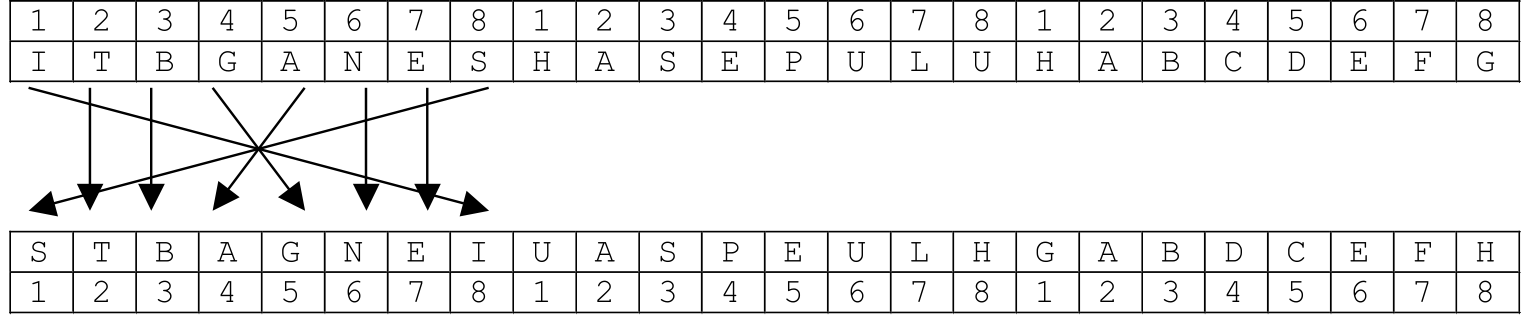
\includegraphics[width=168.00mm,height=89.10mm]{../../images/llm/page_040_img_01.png}%
\end{textblock*}

\end{document}
